\chapter{Pushbroom sensors}
\label{Chap:PushBroom}


%-----------------------------------------------------------------------
%-----------------------------------------------------------------------
%-----------------------------------------------------------------------


%  9 0157  0002 2184 5
%  90157000221845
\section{Notice to the reader}

This chapter present how pushbroom sensors are handled in {\tt MMVII}.
It is written before a programmation session scheduled in mars $2024$
as a support to this session;
it will be probably significantly modified after the session and is different
from the other chapter in two points :

\begin{itemize}
	\item  the  chapter mixes theoreticall aspects with practicall aspects
		of implementation in micmac (some reorganization will probably occur later);
	\item  the theory and organisation are written (at least the first drafts)
               before the actual implementation;
\end{itemize}


%-----------------------------------------------------------------------
%-----------------------------------------------------------------------
%-----------------------------------------------------------------------

\section{Physicall and mathematical modelisation}

%-----------------------------------------------------------------------
\subsection{Physicall model}

\begin{figure}
\centering
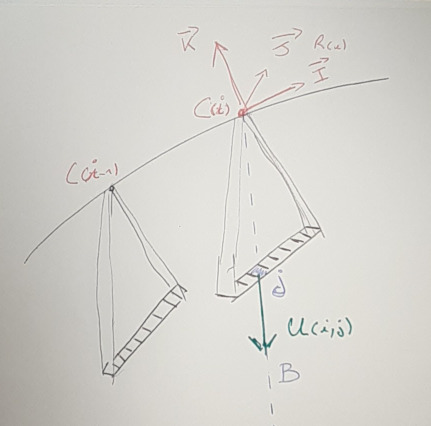
\includegraphics[width=6cm]{Methods/Images/PushB1.jpg}\caption{Notation for pushbroom sensor}
        \label{fig:PushB1}
\end{figure}


A pushbroom sensor is made a monodimensional line sensor which has deplacement during the time.
This is the deplacement that create the second dimension. We suppose in the following  that in the
formed  image the coordinte $j \in [0,n] $ correspond to a line of the monodimensionnal sensor while the coordinate
$i$ correspond to the "time". We note as in figure~\ref{fig:PushB1}:

\begin{itemize}
	\item  $C(t)=C(i)$ the position of the sensor at time $t$;
	\item  $R(t)=R(i)=[\vec{I},\vec{J},\vec{K}]$ the orientation of the sensor at time $t$;
	\item  $\vec{u}(j)$ the direction of bundle in the repair of the sensor;
	\item  $\vec{U}(i,j) = R(i)\vec{u}(j)$ the direction of bundle in the global repair;
	\item  $B(i,j)= (C(i),\vec{U}(i,j))$ the bundle issued of pixel $i,j$;
\end{itemize}

The localisation function is completly caracterized by the mapping $(i,j) \rightarrow B(i,j)$.
By the way, practically we prefer to use the projection $\pi$ that  compute the 
image $i,j$ of given ground point, $\pi : (x,y,z) \rightarrow (i,j)$.  To make
$\pi$ an invertible function we change slightly to $\pi : (x,y,z) \rightarrow (i,j,z)$.
The function "easy" to compute from the previous notation is $\pi^{-1}$,
we have the parametric equation of $B(i,j)(\lambda) = C(i) + \lambda \vec{U}(i,j)$,
and after computing $\lambda$  to have the right $z$ we get :

\begin{equation}
	\pi^{-1}(i,j,z) = C(i) + \frac{z-C_z(i)}{U_z(i)} \vec{U}(i,j)  \label{PushB:EqPiM1}
\end{equation}

The localisation is completely caracterised by :

\begin{itemize}
	\item  the functions $C(i)$ and $R(i)$;
	\item  the calibration of the sensor, i.e. the maping $\mathbb{C}_{al} : j \rightarrow \vec{u}(j)$;
\end{itemize}

%-----------------------------------------------------------------------

\subsection{Non physicall model and reverse engenering}


The equation~\ref{PushB:EqPiM1}, and the devlopment deduced in the following sections,
assume that we have an explicit representation of the physicall parameters
$\mathbb{P}=\{C(i),R(i),\mathbb{C}_{al}\}$.

However , as there is many format that can be fairly complex, it's very
common that the localisation are provided as non physicall model that
give directly access to $\pi$ and $\pi^{-1}$. This the case 
for example with the well known \emph{RPC} format that code
the two function as ratio of polymoms or with the grid-format
(used at \emph{IGN}) that tabulates the values of $\pi$ and $\pi^{-1}$ on grids.

By the way we suppose that we have access, one way or the other,
to the required physicall format because, with a bit of reverse
engeneering, if $\pi$ and $\pi^{-1}$ are accurate enough, it is
still possible to recover them, for example :


\begin{itemize}
	\item the bundle in $B(i,j)$  can be computed as the line $ (\pi^{-1}(i,j,z_1),\pi^{-1}(i,j,z_2)) $
	\item the center $C(i)$ can be computed as the intersection of several bundles $B(i,j_1),(i,j_2) \dots,(i,j_n)$
	\item the axe $\vec{K}$ can be defined as  $B(i,\frac{n}{2})$
        \item the plane containing $\vec{K}$ and $\vec{J}$ can be computed from the set of bundles;
	\item the axe $\vec{I}$ can be computed as $\vec{J} \wedge vec{K}$.
\end{itemize}



%-----------------------------------------------------------------------

\subsection{Satellite model}

Pushbroom sensor are not $100\%$ reserved to satelitte model, they can be used for example for some
aerial camera (see ADS40 frome Leica).
In this chapter we  focuss on satelitte system, this has two consequences :

\begin{itemize}
    \item we assume that $C(i)$  and $R(i)$  are very smooth functions;
    \item we assume that $C(i)$  is known  "perfectly" and that the innaccuracy
          on the model comes only from $R(i)$, and eventualy from the sensor calibration;  this assumption is generally admited
          by the community, as a justification we can give :
    \begin{itemize}
         \item  position comes from GNSS which has a very high accuracy and robustness without obstruction (say a few centimeters);
         \item  orientation comes for stellar sensor, for a saletlite flying at $600km$ at a resolution of $1m$,
                an accuracy of $1$ pixel requires an angular accuracy of $\frac{1}{600000}$ radian or $\frac{1}{10000}$ degree;
     \end{itemize}
\end{itemize}

%-----------------------------------------------------------------------

\subsection{Satellite error model}

\label{PB:SatErMOd}

Let $R(i)$ be the initial orientation , and $R'(i)$ be the "real orientation"
we want to estimate by adjsument.
We admit that there exist a rotation $R_\Theta(i)$, very close to identity and
very smooth so that :

\begin{equation}
    R'(i) = R_\Theta(i) R(i)
\end{equation}

Noting $\Theta=(\omega,\phi,\kappa)$ and as  $R_\Theta$ is close to identity we will have :

%
%
%

\begin{equation}
    R_\Theta(i) = 
\begin{bmatrix}
1 &  - \kappa & \phi\\
\kappa & 1 & -\omega\\
-\phi & \omega & 1
\end{bmatrix} 	
\end{equation}


$\Theta(i)$ will be the unknown we want to compute, but for now
we suppose we know it.  Eventually, later we will add intrinsic calibration
unknown, for example if we add an unknown scaling $\lambda$ to modelize the focal, we will 
have $\Theta=(\omega,\phi,\kappa, \lambda)$

%-----------------------------------------------------------------------

\subsection{Compute projection function with perturbation}

\begin{figure}
\centering
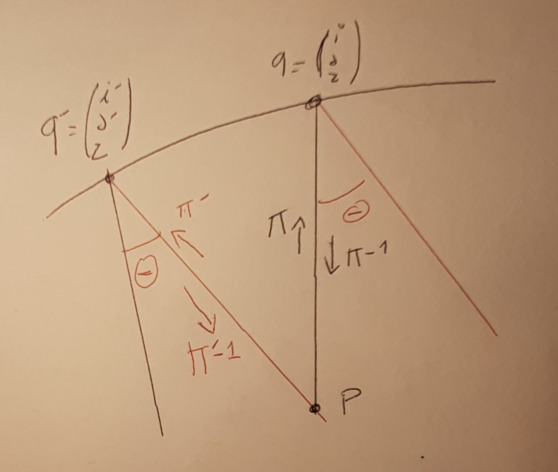
\includegraphics[width=6cm]{Methods/Images/PushB2.jpg}\caption{Notation for perturbated model}
        \label{fig:PushB2}
\end{figure}

We now study how the pertubation model can be integrated in a
computable projection.

Let $\pi$ be the initial projection, we want to compute the modify
projection $\pi'$.
For the invert projection, it's quite obvious, let's note  :

\begin{equation}
    \vec{U'} =  R_\Theta \vec{U}
\end{equation}

Then we have :

\begin{equation}
	\pi'^{-1}(i,j,z) = C(i) + \frac{z-C_z(i)}{U'_z(i)} \vec{U'}(i,j)
\end{equation}


Now for computing $\pi'(P)$ we must compute $q'=(i',j',z)=(i,j,z)+(\delta_i,\delta_j,\delta_z)$ such that :

\begin{equation}
        \pi'^{-1}(q') = P
\end{equation}

Considering $\pi'/\pi'^{-1}$ as a functions of both $q$ and $\Theta$,  we will make a taylor expansion 
of $\pi'^{-1}$. Noting  the jacobians of $\pi'^{-1}$ relatively to $q$ and $\Theta$ :

\begin{equation}
	\mathbb{J}_q(\pi'^{-1}) =
\begin{bmatrix}
       \frac{\partial \pi'^{-1}}{\partial i } &
       \frac{\partial \pi'^{-1}}{\partial j } &
       \frac{\partial \pi'^{-1}}{\partial z } &
\end{bmatrix}
   \; ; \;
      \mathbb{J}_\Theta(\pi'^{-1}) =
\begin{bmatrix}
       \frac{\partial \pi'^{-1}}{\partial \omega } &
       \frac{\partial \pi'^{-1}}{\partial \phi } &
       \frac{\partial \pi'^{-1}}{\partial \kappa } &
\end{bmatrix}
\end{equation}

We can then write the taylor expansion:

\begin{equation}
        \pi'^{-1}(q')
      \approx      \pi^{-1}(q) 
          +   \mathbb{J}_q(\pi'^{-1}) \begin{bmatrix} \delta_i \\ \delta_j \\ \delta_z  \end{bmatrix}
          +   \mathbb{J}_\Theta(\pi'^{-1}) \begin{bmatrix} \omega \\ \phi \\ \kappa  \end{bmatrix}
\end{equation}

But, by definition we have $ \pi'^{-1}(q') =  \pi^{-1}(q) $ so we have :


\begin{equation}
	 \begin{bmatrix} \delta_i \\ \delta_j \\ \delta_z  \end{bmatrix} 
    =  - \mathbb{J}_q ^{-1} \mathbb{J}_\Theta \begin{bmatrix} \omega \\ \phi \\ \kappa  \end{bmatrix}
\end{equation}


We note :
\begin{equation}
	\mathcal{J}(i,j,z) = - \mathbb{J}_q ^{-1} \mathbb{J}_\Theta
\end{equation}

We now have a way to compute $\pi'$ (to first order) : 

\begin{equation}
	 \pi'(P) =  \pi(P)  + \mathcal{J} \begin{bmatrix} \omega \\ \phi \\ \kappa  \end{bmatrix}
\end{equation}

%-----------------------------------------------------------------------

\subsection{Correction model}

As decribed in~\ref{PB:SatErMOd}, we assume that the corrective term between
initial localisation and \emph{real} localisation :

\begin{enumerate}
        \item  is a rotation arround current centers, 
	\item  that this rotation depends only of $i$,
	\item  that it  is very close to identity 
	\item  that it  has very smooth variation.
\end{enumerate}

The small rotation being coded by $\omega,\phi,\kappa$, the classical solution
is to  select a  familly of smooth function and to express them as a linear combinaison
of these smooth function.  Classically we select the polynoms as basis (also other
alternative may be studied later).  So let $N$ be the degree of polynoms,
and $a_i,b_i,c_i$  the coefficient, the projection fonction is :

All these consideration  drive to select for $R(i)$ a pa

\begin{equation}
	 \pi'(i,j,z) =  \pi(i,j,z)  + \sum _{k=0}^{N}  \mathcal{J}(i,j,z)  
                                                \begin{bmatrix} a_k \omega^k \\ b_k \phi^k  \\ c_k \kappa^k  \end{bmatrix}
\end{equation}
%-----------------------------------------------------------------------
\section{Vrac}

\begin{itemize}
    \item begin by example with polynomial image
    \item method with some reverse engenering,  $\pi$ and $\pi^{-1}$ being "black box"
\end{itemize}





